\subsection{Study Evaluation} \label{subsec:evaluation}

% TODO Mehr Interpretation, bisher nur viel Beschreibung

% Wo sind sehr bekannte Gene gelandet? zB TP53, ...
% https://pmc.ncbi.nlm.nih.gov/articles/PMC3527990/#:~:text=The%20most%20relevant%20genes%20in,ALK%2C%20RET%2C%20and%20ROS1.



\begin{figure}[!h]
    \centering
    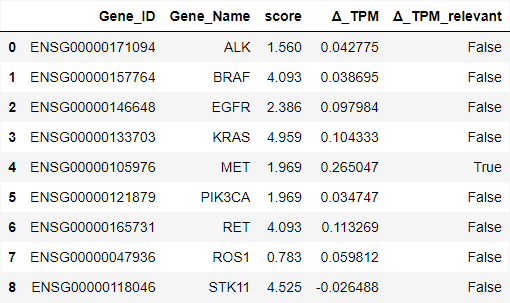
\includegraphics[height=\dfheightdouble]{figures/05_01_df_known_genes}
    \caption{}
    \label{fig:05_01_df_known_genes}
\end{figure}

\begin{figure}[h]
    \minipage{0.45\textwidth}
        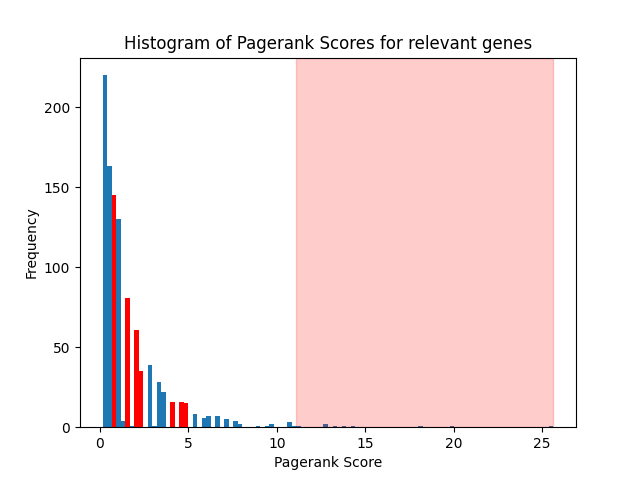
\includegraphics[width=\linewidth]{figures/05_01_pagerank_known_genes}
    \endminipage
    \hfill
    \minipage{0.45\textwidth}
      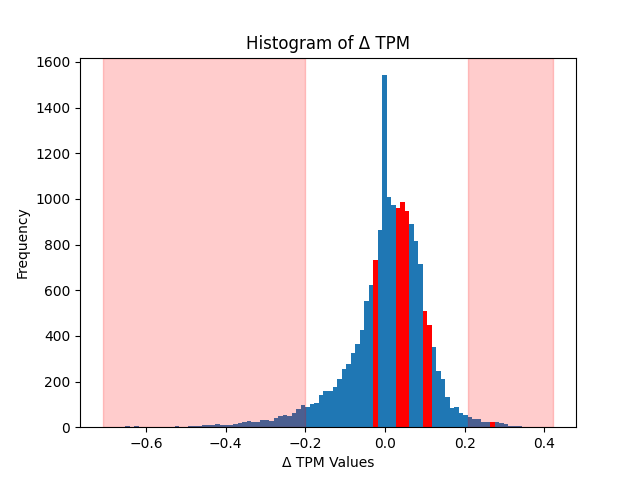
\includegraphics[width=\linewidth]{figures/05_01_delta_tpm_relevant}
    \endminipage
    \caption{Plot of the distribution of the Pagerank score and the $\Delta_{TPM}$ with highlighting of values for known genes}
    \label{fig:05_known_genes}
\end{figure}




% wie kann man Delta TPM einschätzen?


% Wie gut ist der Pagerank?
% Zu viel Gewicht auf den ersten Edges? Quasi nur abhängig von Anzahl der Kanten am Gen - da hätte man sich den Pagerank sparen können



{\color{lightgray}
* Other datasets could be used like TCGA which is common in cancer research \\
* CMP Dataset matched with ENS ID Names might be wrong - would be better to find a good dataset with ens IDs \\
* Other meseares as TPM or an additional?! \\
* relevant delta TMP might be problmeatic - some genes might be more sensitive to smaller changes \\
* Pagerank might be too focused on first level Proteins \\
    % TODO check how pagerank is implemented
}
% Verallgemeinerung der Daten
% gibt keine Inforamtion über Ethnie
% Especially the focus on the older age range may affect the generalizability of our findings to other populations.
